\documentclass[border=4pt]{standalone}
\usepackage{tikz}
\usetikzlibrary{calc}
\begin{document}
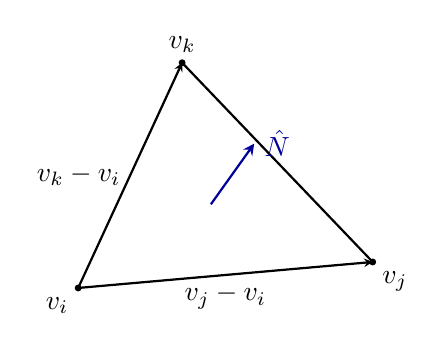
\begin{tikzpicture}[scale=2.2, >=stealth]
  \coordinate (vi) at (0,0);
  \coordinate (vj) at (1.7,0.15);
  \coordinate (vk) at (0.6,1.3);
  \draw[thick] (vi) -- (vj) -- (vk) -- cycle;
  \fill (vi) circle (0.02) node[below left] {$v_i$};
  \fill (vj) circle (0.02) node[below right] {$v_j$};
  \fill (vk) circle (0.02) node[above] {$v_k$};
  \coordinate (centroid) at ($ (vi)!0.333!(vj)!0.333!(vk) $);
  \coordinate (mid) at (0.766,0.483);
  \draw[->, thick, blue!60!black] (mid) -- ++(0.25,0.35) node[right] {$\hat N$};
  \draw[->, dashed] (vi) -- (vj) node[midway, below] {$v_j-v_i$};
  \draw[->, dashed] (vi) -- (vk) node[midway, left] {$v_k-v_i$};
\end{tikzpicture}
\end{document}
